%!TEX program = xelatex
\documentclass[a4paper,12pt]{report}
\usepackage[left=3cm, right=2.5cm, top=2.3cm, bottom=3.5cm]{geometry}
\usepackage{amsmath}
\usepackage{amsfonts}
\usepackage{amssymb}
\usepackage{algpseudocode}
\usepackage{algorithm}
\usepackage{graphicx}
\usepackage[nocomma]{optidef}
% \usepackage{subfigure} % this package will cause error for subfigure, use caption & subcaption instead
\usepackage{caption}
\usepackage{subcaption}
\usepackage{enumerate}         
\usepackage{titlesec}
\usepackage{url}
\usepackage{tocbasic}
\usepackage{color}
\usepackage{tabu}
\usepackage{makecell}
\usepackage[table]{xcolor}
\usepackage[T1]{fontenc}
\usepackage{enumitem}
\usepackage{cite}
\usepackage[redeflists]{IEEEtrantools}
\usepackage[font=small,labelfont=bf]{caption}
\renewcommand{\baselinestretch}{1.5}
\parindent=0pt
\titleformat{\chapter}[block]{\LARGE\bfseries}{\chaptertitlename\ \thechapter}{1em}{\LARGE}

\usepackage{algorithm}
\usepackage{algpseudocode}
\usepackage{graphicx}
\usepackage{amsmath}
\usepackage{gensymb}
\usepackage{textcomp, gensymb}
\usepackage{booktabs,tabularx}
\usepackage{pgfplots}
\usepackage{xurl}
\pgfplotsset{compat=1.10, scaled y ticks=false}
\definecolor{blue}{RGB}{0, 92, 175}
\definecolor{red}{RGB}{208, 16, 76}
\definecolor{green}{RGB}{81, 110, 65}
\definecolor{yellow}{RGB}{255, 177, 27}
\definecolor{brown}{RGB}{86, 46, 55}
\graphicspath{ {./images/} }

\title{Multiple UAV Deployment for Service Time and Throughput Maximization in Disaster Areas\\}
\author{Student: Chen-Yu Yu \\
Advisor: Prof. Sok-Ian Sou\\
\\
Department of Electrical Engineering  \\
National Cheng Kung University \\
Thesis for Master of Science Degree \\
}
\date{July, 2022}

\allowdisplaybreaks[1] 

\begin{document}
\bstctlcite{IEEEexample:BSTcontrol}

\maketitle

\begin{titlepage}
    \begin{center}
        {\bf\large Multiple UAV Deployment for Service Time and Throughput Maximization in Disaster Areas}\\
        {Postgraduate: Chen-Yu Yu \hspace{8mm} Advisor: Prof. Sok-Ian Sou}\\
        {Department of Electrical Engineering}\\
        {National Cheng Kung University}\\
    \end{center}

    \paragraph{}
    \begin{center}
        {\bf Abstract}\\
    \end{center}
    \paragraph{}
    In times of disaster, a flexible and responsive emergency communication network is essential for saving lives and properties, especially after incidents such as hurricanes and floods when terrestrial base stations are not operational. Under such conditions, using unmanned aerial vehicles (UAVs) as aerial base stations is a promising solution due to their agility, mobility, and flexibility. In this work, we deploy multiple UAVs and aim to maximize total user service time while satisfying users' Quality-of-Service (QoS) requirements. Our proposed method divides the target area into several regions based on Voronoi Diagram to effectively serve users under the current distribution of users. By moving circles in each region, we can discover the optimal placement of service areas. Then, we deploy UAVs to service areas with maximum total service time. Our simulation results demonstrate the effectiveness of our approach for achieving higher total service times and fulfilling QoS requirements for users.\\
    
    \textbf{Keywords:} {unmanned aerial vehicle (UAV), aerial base station, 3D deployment, service time, clustering algorithm}
\end{titlepage}

\pagenumbering{roman}
\setcounter{page}{4}
\addcontentsline{toc}{section}{Contents}
\tableofcontents \newpage
\addcontentsline{toc}{section}{List of Figures}
\listoffigures \newpage
\addcontentsline{toc}{section}{List of Tables}
\listoftables \newpage
\pagenumbering{roman}
\setcounter{page}{1}
\pagenumbering{arabic}

%*------------------------------------------------------
\chapter{Introduction}
\paragraph{}
After natural disasters such as earthquakes, floods, and hurricanes, many terrestrial base stations set up by mobile network operators may not remain operational. In the 2011 Great East Japan Earthquake, 4900 base stations stopped working due to the damage from the earthquake or other indirect causes~\cite{b1}. On August 31, 2021, Hurricane Ida in the United States caused 28.1\% of the terrestrial base stations to be out of service in the affected region. In Louisiana, up to 52.1\% are out of service \cite{b2}. These incidents show the vulnerability to service interruptions of current terrestrial networks due to natural disasters. Connectivity outages during natural disasters can cause severe damage to property and human lives. A flexible and effective way of providing emergency communication is needed.
\paragraph{}
A potential solution to this issue is through non-terrestrial networks (NTN). NTN is a three-dimensional (3D) heterogeneous architecture that includes satellites, High Altitude Platform Systems (HAPS), and Unmanned Aerial Vehicles (UAVs) \cite{b3}. These elements allow NTN to provide wide-area connectivity and become an excellent candidate for emergency communication service when terrestrial networks are out of service \cite{b4}. Among satellite communication within NTN, Low Earth Orbiting (LEO) satellites have received massive development and interest (e.g., SpaceX and OneWeb) thanks to the increase in network performance and reduction in manufacturing and launch costs \cite{b5}. Although satellite networks can provide global coverage, it is challenging for ground devices to directly connect with satellites due to the long-distance and limited transmission power. Since UAVs operate at a lower altitude and have flexible connectivity, they can be effectively used to provide emergency communication to ground devices. Compared to terrestrial networks, UAVs have the following features \cite{b6}:
\begin{itemize}
    \item \textbf{Agility:} With the ability to move swiftly, UAVs can provide on-demand communication and quick responses to the current environment under different conditions. This characteristic brings additional degrees of freedom when dealing with user distribution changes.
    \item \textbf{Mobility:} UAVs can move along any trajectory with a lesser chance of encountering obstacles. They can also be deployed in high-risk environments and rural areas since they can be remotely controlled and don't require drivers.
    \item \textbf{Flexibility:} UAVs operate in 3D space with adjustable height, making them more likely to overcome signal blockage and establish LoS connections with ground devices. As a result, the coverage, capacity, and latency of the network provided by UAVs can be improved.
\end{itemize}
\paragraph{}
Although there are many benefits for UAVs in providing communication services, deploying UAVs will face some challenges. For instance, UAV's pathloss depends not only on the user's location but also UAV's flying altitude. Pathloss does not rise or fall linearly due to signal blockage or reflection by objects and the distance between the sender and receiver \cite{b7}. For UAVs to effectively communicate with ground devices, selecting the correct flying altitude under the current placement is essential for UAVs. In \cite{b8} gives an air-to-ground channel model considering propagation conditions under different environments. The model can be used to find the optimal UAV flying altitude in terms of service area radius.
\paragraph{}
For UAVs to serve users effectively, it is crucial to create service areas according to user distribution. In \cite{b9} proposes a solution using K-means clustering and Voronoi Diagram to partition ground users into several convex regions. With the help of the Voronoi Diagram, we can discover user centroids and place service areas in convex regions. Moreover, boundary lines created by convex regions can ensure service areas will not overlap, preventing inter-cell interference between UAVs.
\paragraph{}
Under a normal situation, users will not always stay at the same location. Users might move along a path to a random waypoint (e.g., random waypoint model) \cite{b10}. After some time, UAV will have to move to a new location to serve more users. However, the UAV's movement will let users suffer from fast fading and Doppler effects, which cause unstable connections when UAVs are traveling. We exploit in-service time \cite{b11} to indicate the time available to serve users. A user's in-service time is derived by subtracting the travel time of the serving user's UAV from the user's sojourn time, where the sojourn time is the expected duration the user will stay at the same location. Travel time for the UAV will vary based on the current location and the desired destination. If moving farther away, the in-service time will decrease. There may be a trade-off between moving to a distant location to serve more users with a longer total sojourn time and moving to a closer location but serving fewer users. In addition to in-service time, users' throughput requirement is essential when providing communication services. Signal coverage does not always guarantee acceptable network performance \cite{b12}. Although web browsing is widely used, according to \cite{b13}, video streaming now consumes over half of the global bandwidth. With the ability to watch and stream videos in disaster areas, doctors can perform remote medical treatment, and people can receive and report incidents more effectively.
\paragraph{}
In this paper, we study the deployment of UAVs as aerial base stations in 3D to provide communication services for users located in coverage holes. Following the work of \cite{b14} and \cite{b15}, we assume that the position of all users is available through high-accuracy Global Positioning Systems (GPS). We utilize rotary-wing UAVs for deployment as aerial base stations that can hold still in the air. Our aim is to maximize the service time provided by UAVs and ensure that all users served can receive a minimum amount of throughput. The main contributions are summarized as follows:
\begin{itemize}
    \item To jointly consider in-service time and user's QoS requirement, we maximize total in-service time while guaranteeing each user's QoS requirement. As a result, we can maximize the time users are served by UAVs while also meeting users' demand for Internet access.
    \item We propose Dynamic Service Area (DSA) algorithm to deploy UAVs effectively. The algorithm will first generate service areas as UAV deploying location candidates. DSA optimizes service areas by moving and increasing the radius within each convex region to find the optimal size and placement that offers the maximum amount of in-service time while meeting each user's QoS requirements. Each service area's height is determined by the maximum throughput possible given the distance between the users and the UAV. UAVs will then be deployed to service areas that can provide maximum total in-service time. After a given interval, UAVs' placement will be adjusted based on the dynamic analysis of service areas in response to the current user distribution.
    \item We use practical simulations and settings to study the performance of our proposed method and compare it with different algorithms and parameters. Our simulation results demonstrate the effectiveness of our approach by considering in-service time and satisfying each user's QoS requirement through service area optimization.
\end{itemize}
\paragraph{}
The rest of the paper is organized as follows. In Chapter~2, we review related works. Then, we introduce the system model in Chapter~3. Our proposed method will be introduced in Chapter~4. Finally, we report our performance evaluation in Chapter~5 and draw our conclusion in Chapter~6.

%*------------------------------------------------------

\chapter{Related Work}
\paragraph{}
The problem of finding optimal deployment and trajectory of multiple UAVs has been studied extensively to improve network coverage and performance. For instance, Sun et el. \cite{b14} utilize Voronoi Diagram and proposed the SD-KMVR algorithm to maximize user coverage and power efficiency. The proposed method seeks the optimal placement of user coverage areas by shrinking and moving them from the maximum allowed radius. By ensuring users' QoS requirement while considering co-channel interference when deploying multiple UAVs, in \cite{b15} proposes a solution to maximize throughput by optimizing UAV's altitude and transmit power. For the continuous movement of users, the authors in \cite{b16} propose a machine learning-based approach. At first, the initial user partition is given by the GAK-means algorithm. Then a Q-learning algorithm is applied to adapt to users' movement and decide the 3D deployment of UAVs. In \cite{b17} aim to maximize service time under limited energy by minimizing the energy consumption used by the trajectory of UAVs.
\paragraph{}
As for utilizing UAVs to provide communication service under emergencies, in \cite{b18} UAVs are used in disaster areas to restore communication and maintain network connectivity. The authors develop a K-means clustering-based algorithm that considers the decision time and energy efficiency needed to provide optimal resource allocation. In \cite{b19} the authors focus on conveying emergency messages in coverage holes with UAV. The proposed algorithm considers the trajectory of UAVs to send messages with the shortest mission completion time. The work in \cite{b20} integrates UAVs and LEO satellites in emergency areas without ground facilities to meet the QoS requirements of different users. The proposed solution optimizes the 3D location, power, and bandwidth of UAVs.
\paragraph{}
The cost of UAV travel and the continuous movement of ground users are rarely considered in UAV deployment problems. However, UAV's travel time and user's sojourn time are two major factors that will affect a user's service time. In the worst-case scenario, UAV might not serve any user when it moves to a new location since all users have already left, which results in a waste of the already limited onboard UAV resource and potential to serve other users. On the other hand, each user's QoS requirement is also a major factor in UAV deployment. Users would like to send and receive new information on their devices. In this paper, we will address this problem through our proposed approach by using the in-service time and meeting users' QoS requirements.

%*------------------------------------------------------

\chapter{System Model}
\section{System Description}
\paragraph{}
We consider a square area with a set of terrestrial base stations $T$ remaining working after the disaster. Each terrestrial base station has a static serving radius. The whole area is divided into $R$ regions, and each region contains a service area to determine the candidate location of UAVs. Each service area $s$ has coordinates $(x_{s},y_{s},z_{s}), s = 1, 2, \ldots, R$ and radius $b_{s}, s = 1, 2, \ldots, R$. We assume a finite number of aerial base station-equipped UAVs are available for deployment. A set of UAVs $W$ with 3D coordinates $c_w, w = 1, 2, \ldots, W$ will be initialized at (0, 0, 0) and will not omit signal while moving. Since the objective is to deploy UAVs in places without signal coverage, UAVs will avoid deploying to areas that can still receive communication service from terrestrial base stations. Each UAV will only hover above one service area at a time. We assume all UAVs can move along the shortest path and will not encounter any obstacles along the way. UAVs will redeploy only after the given deployment interval to avoid unnecessary movement and preserve energy.

\begin{figure}
    \centering
    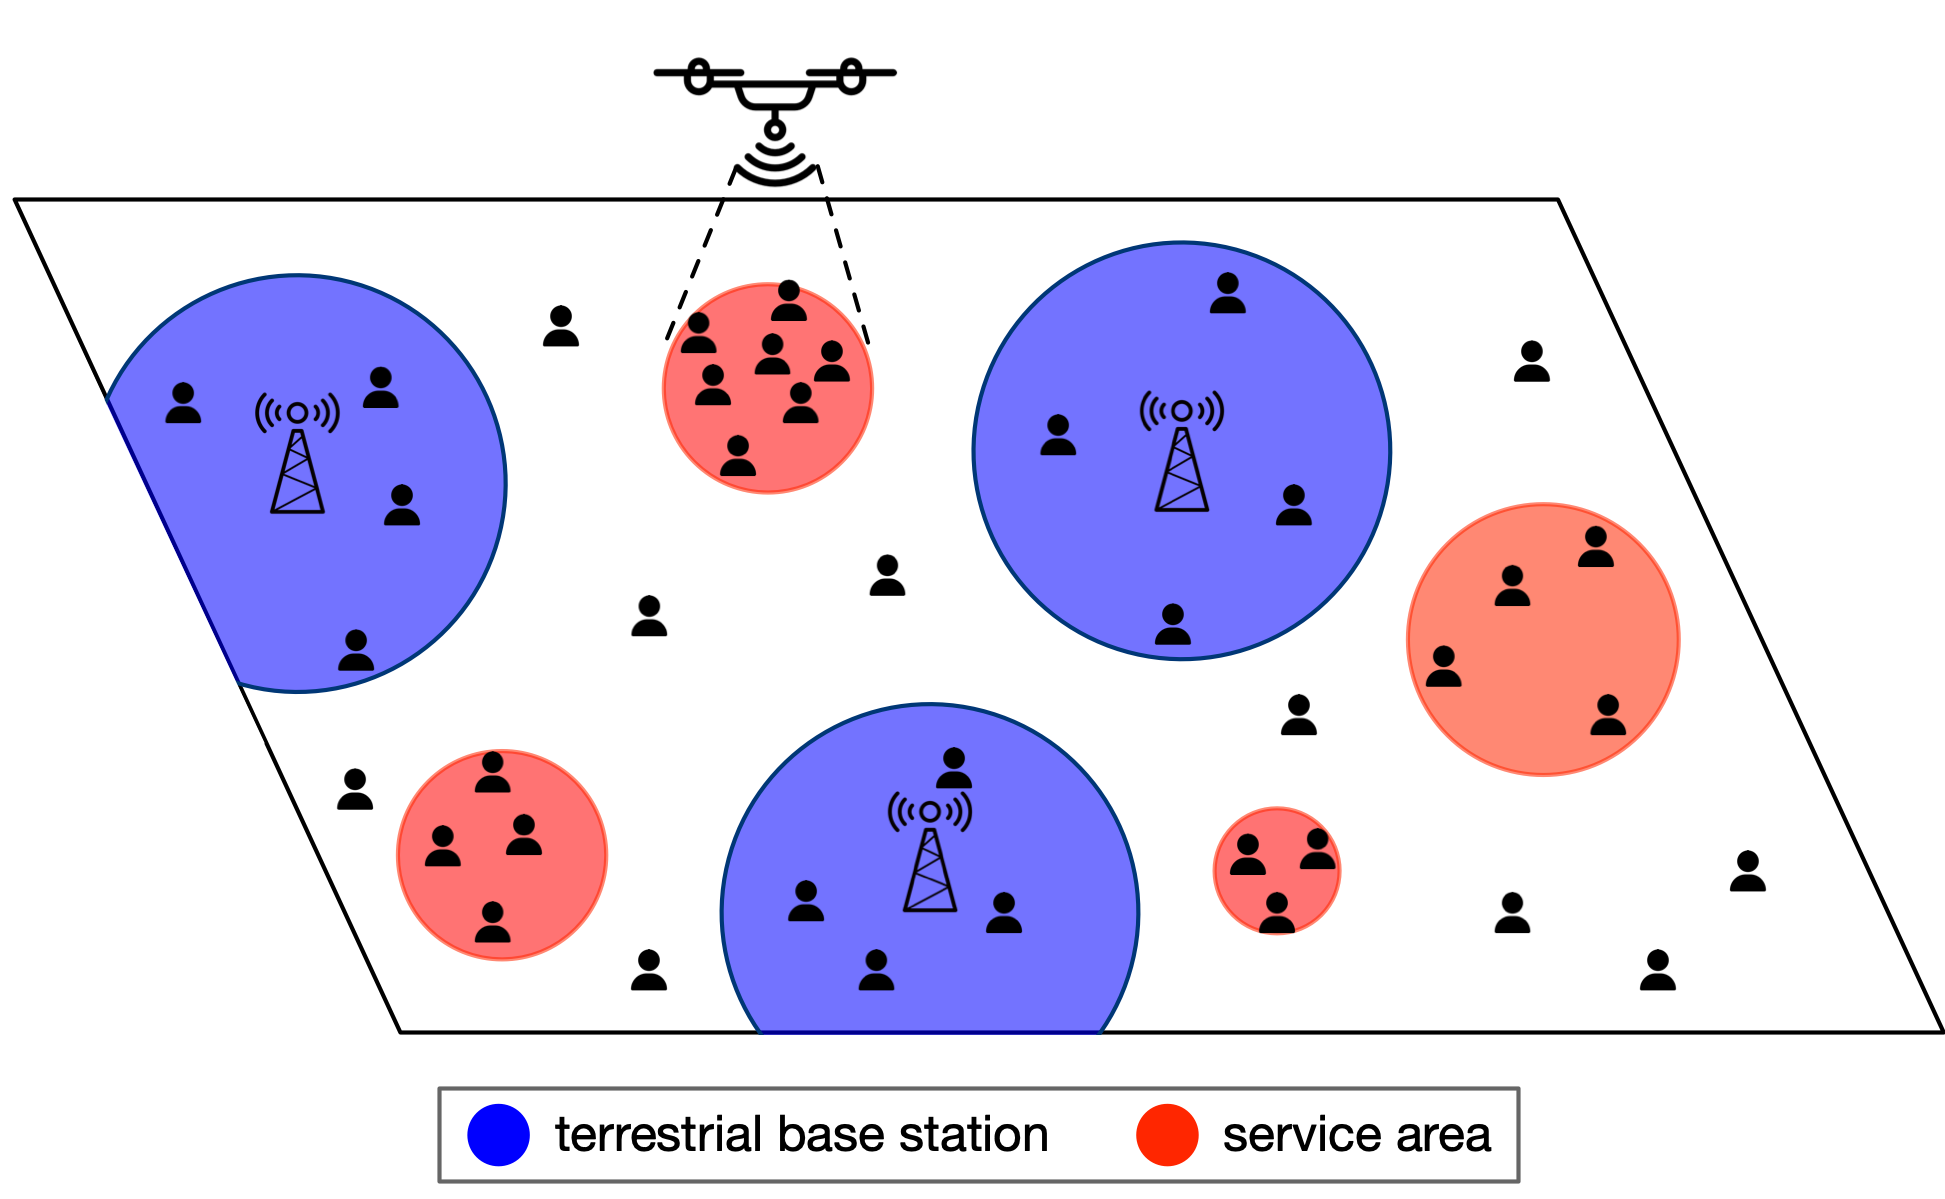
\includegraphics[width=0.8\textwidth]{Figure 1.png}
    \caption{An illustration of the system model.}
    \label{fig:System Model Example}
\end{figure}

\paragraph{}
Inside the square area also contains a set of users $U$, where we assume each user $u$'s coordinates $(x_{u},y_{u},z_{u}), u = 1, 2, \ldots, U$ is known and has a QoS requirement $t_{u}$, $u = 1, 2, \ldots, U$ with an estimated sojourn time $s_{u}$, $u = 1, 2, \ldots, U$. The sojourn time for each user will not exceed the deployment interval. When a user's sojourn time ends, the user will start moving to its next location and have a new sojourn time after arriving at the new destination. Each UAV $w$ has a limited user serving capacity $N$, and each user will only be served by at most one UAV at a time. If UAV $w$ is moving from $c_{w}$ to $\hat{c_{w}}$ with a travel time $t_{w}(c_{w}, \hat{c_{w}})$ to serve user $u$, user $u$'s in-service time $i_{u}$ is $max\{0, s_{u} - t_{w}(c_{w}, \hat{c_{w}})\}$. An illustration of the complete system model is given in Fig.~\ref{fig:System Model Example}.

\section{Channel Model}
\paragraph{}
Users will generally experience two kinds of signals from UAVs including LoS and Non-Line-of-Sight(NLoS) connections. The LoS probability is given in \cite{b8} as follows:
\begin{equation}
    P(LoS)=\frac{1}{1+a\;exp(-b(\frac{180}{\pi}\theta - a))}
\end{equation}
where $\theta=arctan(\frac{h}{r})$ is the elevation angle between the UAV and user. $h$ is UAV's flying height and $r$ is the service area's radius. $a$ and $b$ are positive constants that depend on the environment. The probability of NLoS can be referred to as P(NLoS)=1 - P(LoS). With the probability of both LoS and NLoS channels, the mean pathloss model (dB) for user $u$ served by UAV $w$ can be expressed as \cite{b7}:
\begin{equation}
    \begin{aligned}
    PL_{u} & = 20log_{10}(\frac{4\pi f_{c}d}{c})\\
    &\quad +P(LoS)\eta _{LoS}+P(NLoS)\eta _{NLoS}
    \end{aligned}
\end{equation}
where $f_{c}$ is the carrier frequency (Hz), $d$ is the distance from UAV $w$ to user $u$, and $c$ is the speed of light (m/s). $\eta _{LoS}$ and $\eta _{NLoS}$ (in dB) are the average additional losses corresponding to LoS and NLoS links.

\begin{figure} [t!]
    \centering
    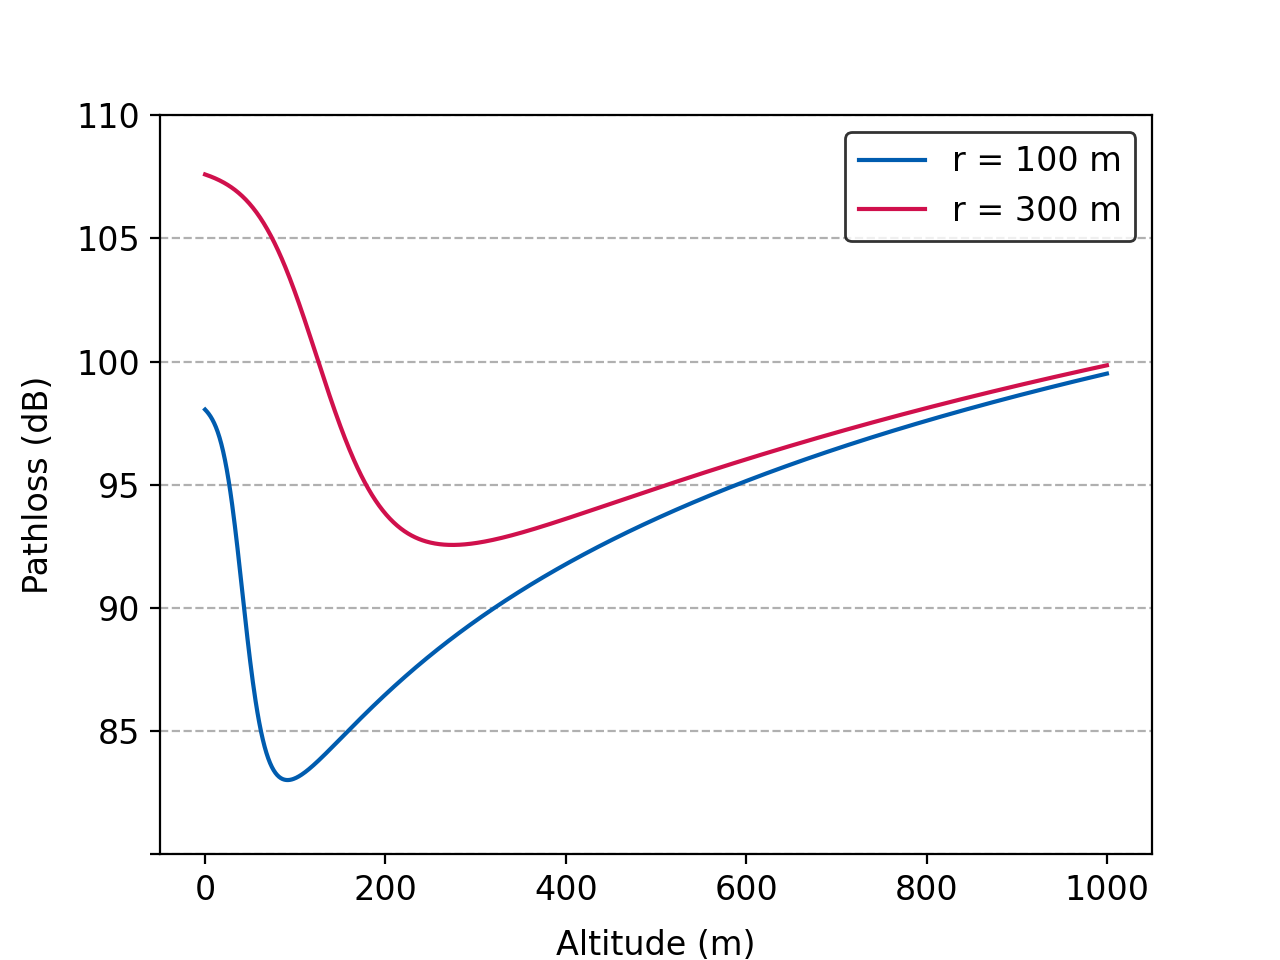
\includegraphics[width=0.75\textwidth]{Figure 2.png}
    \caption{Impact of pathloss under different UAV flying altitudes with two service area radii.}
    \label{fig:Pathloss vs Altitude}
\end{figure}

\paragraph{}
Figure~\ref{fig:Pathloss vs Altitude} shows the impact of pathloss under different UAV flying altitudes in an urban environment. As shown in this figure, pathloss decreases from a larger value and increases again after reaching a certain height as the flying height increases. At first, pathloss starts at a greater value since there is a higher chance of encountering Non-Line-of-Sight (NLOS) than LoS due to object reflections such as buildings at low flying levels. As flying height increases, connections are less likely to be obstructed by objects and increase the probability of LoS, which contributes to the decrease of pathloss. However, after reaching a certain altitude, although LoS dominates most connections, the pathloss will increase as the distance between the transmitter and receiver increases \cite{b7}\cite{b8}. As a result, we can achieve optimal connections with ground devices by selecting the correct flying height for the serving UAV based on the service area radius.
\paragraph{}
Our system considers the total bandwidth is distributed equally among ground devices served by the same UAV. Following the Shannon capacity theorem, user $u$'s data rate (bits/second) provided by UAV $w$ data rate can be expressed as follows: \cite{b21}:
\begin{equation}
    r_{u} = \frac{B}{|U_{w}|}\;log_{2}(1+\frac{P_{u}}{10^{PL_{u}/10}\cdot{\sigma ^{2}}})
\end{equation}
where $B$ is the bandwidth available for a UAV and $|U_{w}|$ is the number of users served by UAV $w$. $P_{u}$ is the power allocated to the user $u$, and $\sigma ^{2}$ is the power of the white Gaussian noise.
\paragraph{}
The list of notations given in two subsections is summarized in Table~\ref{table:Summary of Notation}.

\begin{table} [h!]
    \centering
    \caption{Summary of notations}
    \label{table:Summary of Notation}
    \begin{tabularx}{\linewidth}{c X}
    \toprule
    \textbf{Symbol} & \textbf{Description}\\
    \midrule
    \\ [-2em]
    $T$                             & The set of terrestrial base stations                     \\ [0.5ex]
    $R$                             & The set of regions                                       \\ [0.5ex]
    $(x_{s},y_{s},z_{s})$           & The coordinates of service area $s$                      \\ [0.5ex]
    $b_{s}$                         & The radius of service area $s$                           \\ [0.5ex]
    $Sc$                            & The set of service area coordinates                      \\ [0.5ex]
    $W$                             & The set of UAVs                                          \\ [0.5ex]
    $c_w$                           & UAV $w$'s coordinates                                    \\ [0.5ex]
    $N$                             & UAV's serving capacity                                   \\ [0.5ex]
    $U$                             & The set of users                                         \\ [0.5ex]
    $(x_{u},y_{u},z_{u})$           & User $u$'s coordinates                                   \\ [0.5ex]
    $t_u$                           & User $u$'s QoS requirement                               \\ [0.5ex]
    $s_u$                           & User $u$'s sojourn time                                  \\ [0.5ex]
    $i_u$                           & User $u$'s in-service time                               \\ [0.5ex]
    $r_{u}$                         & Data rate served by UAV $w$ to user $u$                  \\ [0.5ex]
    $P_u$                           & Power allocated for user $u$                             \\ [0.5ex]
    $f_c$                           & Carrier frequency                                        \\ [0.5ex]
    $B$                             & Bandwidth available for a UAV                            \\ [0.5ex]
    $l_r$                           & Boundary lines of region $r$                             \\ [0.5ex]
    \bottomrule
    \end{tabularx}
\end{table}

\chapter{In-Service Time based 3D UAV deployment with QoS awareness}
\paragraph{}
To achieve our goal of maximizing total in-service time while satisfying users' QoS requirements with a limited number of UAVs, we propose DSA. DSA involves two steps, where we will first create service areas and then deploy UAVs. Due to the repositioning of service areas and redeployment of UAVs based on the snapshot of current user distribution in every deployment interval, the DSA algorithm is considered an offline algorithm. The flow chart of DSA is shown in Figure~\ref{fig:DSA Block Diagram}. In the following subsections, we will discuss the methods used in each step.

\begin{figure} [ht]
    \centering
    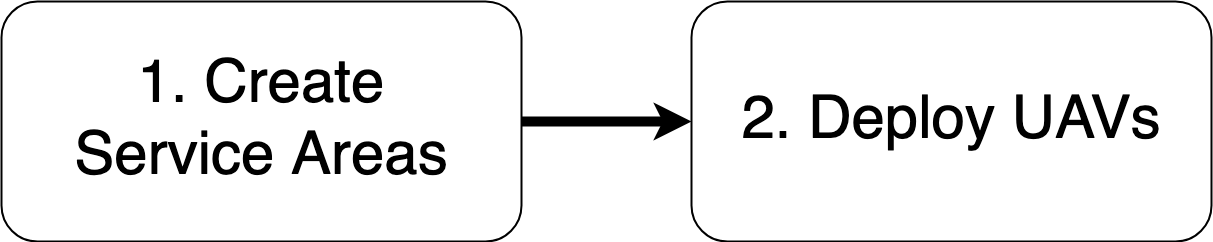
\includegraphics[width=0.6\textwidth]{Figure 3.png}
    \caption{Block diagram of the proposed Dynamic Service Area Algorithm.}
    \label{fig:DSA Block Diagram}
\end{figure}

%*------------------------------------------------------

\section{Create Service Areas}
\paragraph{}
By creating service areas, we can conveniently identify possible placements within the 3D space that meet our objectives. However, finding the optimal placement and size of service areas is not a trivial problem and will seriously impact the performance of our goal. As users' location in the network changes over time, service areas' placement has to update accordingly to provide maximum in-service time. On the other hand, service areas' radius and height must also be optimized to meet users' QoS requirements. If the service area has a radius too large, some users might be too far away from the UAV, which makes meeting these users' QoS requirements more challenging. Moreover, as more users may be served within a greater radius, it may be more difficult to satisfy all users' QoS needs since the bandwidth is shared. By contrast, a small service area might only serve a few users. This may result in the UAV not reaching its service capacity, but serving fewer users and reducing the in-service time it may be able to provide.
\paragraph{}
Before generating service areas, it will be beneficial to cluster all users in the network to serve as many users as possible. Through clustering, the distribution of users can be discovered, such as where users are more densely populated and also find out the centroid of users in each cluster. As for our clustering method, we use the well-known and popular K-means clustering. We divide users into $R$ clusters and form the Voronoi diagram. Inside the Voronoi diagram contains several regions formed by a set of boundary lines $l_r , r = 1, 2, \ldots, R$. The UAV deployment problem can be substantially simplified by placing service areas in each region so they will not overlap, thus preventing inter-cell interference caused by deploying multiple UAVs.
\paragraph{}
Since users will leave their current location after their sojourn time ends, the overall user distribution may change over time after each user movement. The change in user distribution may cause the creation of new user clusters, and these clusters will change their size and location over time. To determine the optimal placement and radius of service areas with the current user distribution after every deployment interval, we will move each service area within its region to ensure maximum in-service time. We will also obtain the appropriate height of service areas with minimum pathloss by the distance between the serving users and the UAV. It is also crucial that service areas are placed so they can meet the QoS requirements of every serving user and not exceed the serving capacity of each UAV. The optimization problem of creating service areas can be formulated as the following:
\begin{maxi!}|l|[2]
    {x_s,y_s,z_s,i_u}{I_{sum} = \sum_{u=1}^{U}{i_{u}c_{u}}}                    {\label{op}}{\nonumber}
    \addConstraint{r_u \geq t_u, \ \forall u \in U,                             \label{op:con1}}
    \addConstraint{c_u \in \left \{ 0,1\right \},\ \forall u \in U,             \label{op:con2}}
    \addConstraint{|c_u| \leq N,\ \forall c_u = 1,                              \label{op:con3}}
    \addConstraint{(x_s-l_r)^{2}+(y_s-l_r)^{2}\geq bs^{2},\ \forall r \in R     \label{op:con4}}
\end{maxi!}
where constraint (\ref{op:con1}) is to ensure all users served by the UAV will satisfy their QoS requirement. Constraint (\ref{op:con2}) indicates the serving status of user $u$, while $c_u = 1$ denotes user $u$ is served by this service area and $c_u = 0$ does not. As UAVs have a limited number of users they can serve, constraint (\ref{op:con3}) ensures UAVs will only serve users under their serving capacity $N$. Considering that service areas can only move within their respective regions, constraint (\ref{op:con4}) verifies whether the current service area is within boundary lines.

\section{Deploy UAVs}
\paragraph{}
After having a list of service areas, we can then deploy UAVs to different service areas. To follow our goal, we will first find the placement with maximum in-service time from all available service areas, then assign the corresponding UAV to the optimal location. As one region only hovers one UAV, we will remove that region from other UAVs to prevent users from being served by multiple UAVs. This process will repeat until there are no UAVs left undeployed.

\section{Dynamic Service Area Algorithm}
\paragraph{}
Algorithm~\ref{alg:DSA} is the pseudocode of the proposed DSA algorithm. First, in Line~1, list $L$ is initialized to collect the information of all service areas for all UAVs. Since UAVs will not deploy to areas where terrestrial base stations remain operational, Line~2 will remove all terrestrial base stations' coverage areas in all regions. Line~3-21 is the segment for creating service areas. The algorithm will generate service areas for all UAVs in all regions since each UAV's current location might be distinct (Lines~3-4). To know the maximum radius available, we calculate $b_{max}$ for the maximum radius in this region (Line 5). In Line~6 and 7, we initialize $b_s$ with $b_i$ to track the current radius of the service area, and also $I_{best}$ to save the most optimal in-service time result. From Line 11 through 17, the algorithm checks every possible placement of the service area until reaching the maximum possible radius in the region. Circle $c$ will be formed with the current radius $b_s$ (Line 9). In Line~10, with circle $c$, we can obtain the optimal placement of the service area in ($x_s, y_s, z_s$) that has maximum in-service time $I_{sum}$ by solving the optimization problem (\ref{op}). From Line 11 to 16, if $I_{sum}$'s in-service time is larger than the previous best in-service time $I_{best}$, we will save $I_{sum}$ as the new best in-service time and increase $b_{s}$ for the next round. If $I_{sum}$'s in-service time is less than or equal to $S_{best}$, it shows that we have already found the optimal placement and in-service time result, which indicates we can break the while loop. The final coordinates of the service area are then saved to $c_s$ (Line~18). Results including the current UAV, the service area coordinates, and the in-service time will be added to the list $L$ (Line~19). From Lines~22 to 27 is the deployment for all UAVs. By examining list $L$, we find the service area located at $c_m$ with the maximum in-service time provided by UAV $w$ (Line~23). We then assign UAV $w$'s deploying location as $c_m$ (Line~24). Since UAV can only serve one location, we remove UAV $w$ from list $L$ (Line~25). As one region can also be served by one UAV, we will also remove service area $s$ from list $L$ (Line~26). Finally, in Line 20, we return the new deploying coordinates $\hat{c_{w}}$ for all UAVs $W$. An example result of the Dynamic Service Area Algorithm is shown in Figure~\ref{fig:DSA example}.
\begin{figure} [h!]
    \centering
    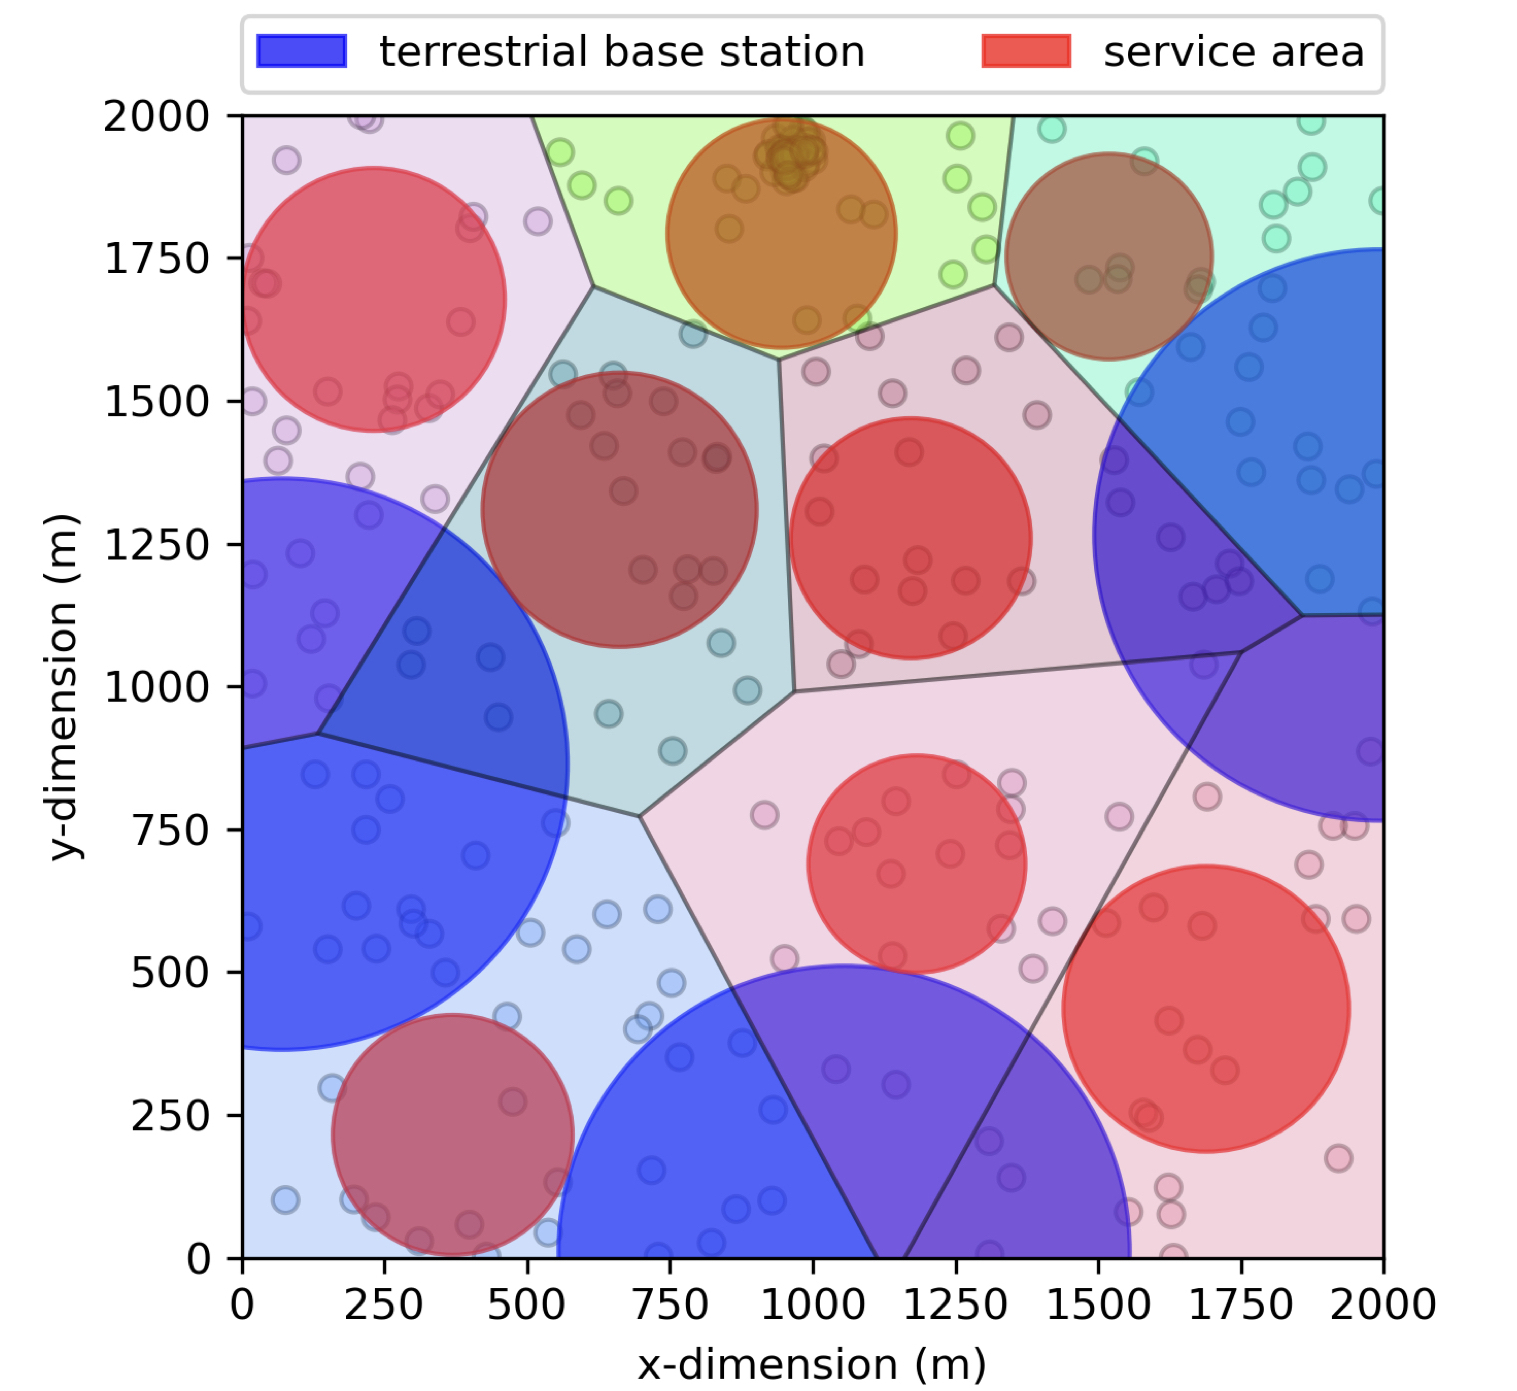
\includegraphics[width=0.7\textwidth]{Figure 4.png}
    \caption{An example result of the proposed Dynamic Service Area Algorithm.}
    \label{fig:DSA example}
\end{figure}
\begin{algorithm}[t!]
    \caption{Dynamic Service Area Algorithm}
    \label{alg:DSA}
    \algrenewcommand\algorithmicrequire{\textbf{Input:}}
    \algrenewcommand\algorithmicensure{\textbf{Output:}}
    \begin{algorithmic}
    \Require $W, R, U$, Initial radius $b_{i}$
    \Ensure $\hat{c_{w}}$, $\forall w \in W$
    \State $L \gets \emptyset$
    \State Remove $T$ in $R$
    \ForAll {$w \in W$}
        \ForAll {$r \in R$}
            \State Calculate maximum radius $b_{max}$ in region $r$
            \State Initialize $b_s$ with $b_i$
            \State $I_{best} \gets 0 $
            \While{$b_{s} \leq b_{max}$}
                \State Form circle $c$ with radius $b_{s}$
                \State Obtain $(x_s, y_s, z_s)$ and $I_{sum}$ from solving (\ref{op})
                \If{$I_{sum} > I_{best}$}
                    \State $I_{best} \gets I_{sum}$
                    \State Increase $b_{s}$
                \ElsIf{$I_{sum} \leq I_{best}$}
                    \State break
                \EndIf
            \EndWhile
            \State $c_s \gets (x_s, y_s, z_s)$
            \State $L \gets L \cup \left \{ w, c_s, I_{best} \right \} $
        \EndFor
    \EndFor
    \While{$L \neq \emptyset$}
        \State From $L$ find maximum in-service time $i_u$ at $c_m$ by $w$
        \State $\hat{c_{w}} \gets c_m$
        \State Remove $w$ from $L$
        \State Remove $c_m$ from $L$
    \EndWhile
    \State \Return $\hat{c_{w}}$, $\forall w \in W$
    \end{algorithmic}
\end{algorithm}
%*------------------------------------------------------

\chapter{Performance Evaluation}
\section{Simulation Setups}
\paragraph{}
We evaluate our Dynamic Service Area Algorithm by comparing it with two algorithms. The first algorithm is \mbox{SD-KMVR} which is proposed in \cite{b14}. SD-KMVR will place user coverage areas in each region formed by the Voronoi Diagram to serve the maximum amount of users. By moving and shrinking the circle from the largest radius available in each region, the algorithm finds the most optimal placement of coverage areas. Every user coverage area's height in SD-KMVR is determined with \begin{equation}\label{SD-KMVR height}
    h_s = \frac{b_s}{tan(\frac{\theta _B}{2})}
\end{equation}
where $\theta_B$ is the antenna beamwidth of UAV and $h_s$ is the height of user coverage $s$. Another algorithm we utilize for comparison is the Mobile Small-Cell Deployment (MSCD) Algorithm \cite{b12}. MSCD focuses on maximizing in-service time with several mobile small cells. It uses randomly generated predefined locations with a fixed placement and radius for mobile small cells to select their target locations. As MSCD is originally an algorithm that considers deployment for mobile small cells in 2D, we will select each predefined location's height by their corresponding radius with the optimal height in our channel model.
\paragraph{}
For our UAV deploying environment, we consider a 2000~m$^2$ sized square area located in an urban area. According to \cite{b8}, the corresponding parameters in urban area for our channel model are $(a, b)=(9.61, 0.16)$ and $(\eta _{LoS}, \eta _{NLoS})=(1, 20)$. The carrier frequency $f_c$ is 2~GHz, and the available bandwidth $B$ for each UAV is 20~MHz. Each user served by the UAV is allocated with a power of $P_u = 15$~dBm.
\paragraph{}
There are three terrestrial base stations that remain operational within the area, each having a service radius of 500~m. We will create eight service areas and three UAVs available for deployment. According to \cite{b22}, the communication-related power consumption in a UAV is specified as 5~W. Given the communication-related power and each user's allocated power, the maximum serving capacity $N$ can be derived as 158~users. Each UAV has a maximum flying altitude of 300~m \cite{b23} and a moving speed of 10~m/s. Based on UAV's moving speed, the deployment interval of UAVs is 300~s.
\paragraph{}
Users are randomly generated in the simulation area with a moving speed of 1~m/s. We assume all users will move with the random waypoint mobility model \cite{b10}. Some users will be aggregated in hotzones such as shelters in disaster areas. There will be one hotzone located in the system with a radius of 50~m. For the number of users in each hotzone, we refer to the hotzone model given in \cite{b24}. The formula is shown as follows:
\begin{equation}
    N_{s} = \left\lfloor p\;\cdot\frac{|U|}{|W|} \right\rfloor
\end{equation}
where $N_{s}$ is the number of users who stay in a particular hotzone, and p is the ratio of users who stay in a particular hotzone compared to the total number of users. The total number of users and UAVs inside the network are indicated by $|U|$ and $|W|$. There will only be a few users leaving the hotzone that might be paramedics or members of the rescue team. Other users located in the hotzone will remain inside. Even though some users are aggregated in hotzone areas, additional clustering areas may be created after user movement. These newly formed clusters will change in size and location over time. We will utilize the DSA algorithm to discover the optimal placement of service areas to deploy UAVs.
\paragraph{}
For users' QoS requirements, we consider users will generally have two types of requirements. One is web browsing, and the other is video streaming. With the ability to achieve video streaming, users can report or receive the latest information on the current situation, and the rescue team can perform remote medical treatments \cite{b25}. According to FCC's broadband speed guide \cite{b26}, the recommended minimum download speed for web browsing is 1~Mbps and 3~Mbps for video streaming. For users' QoS requirements ratio, 30\% of users will require video streaming, and the rest will only need web browsing. Each user's QoS requirement will be renewed after every deployment interval.
\paragraph{}
The given parameter settings are summarized in Table~\ref{table:Parameter Settings}. We obtain our simulation result with an average of 100 consecutive runs.

\begin{table} [t!]
    \centering
    \caption{Parameter settings}
    \label{table:Parameter Settings}
    \begin{tabularx}{0.65\linewidth}{l c}
    \toprule
    \textbf{Parameter} & \textbf{Value}\\
    \midrule
    \\ [-2em]
    Simulation area                                     & 2000 $\times$ 2000~m$^2$            \\ [0.5ex]
    $a$, $b$, $\eta _{LoS}, \eta _{NLoS}$ \cite{b8}     & 9.61, 0.16, 1, 20                   \\ [0.5ex]
    Carrier frequency $f_c$                             & 2 GHz                               \\ [0.5ex]
    Bandwidth $B$                                       & 20 MHz                              \\ [0.5ex]
    Power per user $P_u$                                & 15 dBm                              \\ [0.5ex]
    Communication-related power \cite{b22}              & 5 W                                 \\ [0.5ex]
    Number of terrestrial base stations                 & 3                                   \\ [0.5ex]
    Terrestrial base station radius                     & 500~m                               \\ [0.5ex]
    Number of users                                     & 250-2000                            \\ [0.5ex]
    Number of service areas                             & 4-12                                \\ [0.5ex]
    Number of UAVs                                      & 1-5                                 \\ [0.5ex]
    UAV serving capacity $N$                            & 158 users                           \\ [0.5ex]
    UAV antenna beamwidth $\theta_B$ \cite{b14}         & 95$^{\circ}$                        \\ [0.5ex]
    Maximum UAV flying altitude \cite{b23}              & 300~m                               \\ [0.5ex]
    Web browsing QoS Requirement \cite{b26}             & 1 Mbps                              \\ [0.5ex]
    Video streaming QoS Requirement \cite{b26}          & 3 Mbps                              \\ [0.5ex]
    Deployment interval                                 & 300~s                               \\ [0.5ex]
    \bottomrule
    \end{tabularx}
\end{table}

\section{Simulation Results}
\paragraph{}
Figure~\ref{fig:Impact on Total In-service Time} compares the total in-service time provided under different numbers of users with three algorithms. DSA outperforms the other two algorithms across different numbers of users. This is due to DSA focusing on maximizing users' in-service time, whereas SD-KMVR only considers serving the maximum amount of users. Although MSCD also considers the in-service time when deploying UAVs, having static predefined locations prevent it from serving users effectively when users are mobile. In our proposed DSA algorithm, the total in-service time rises when the number of users increases since more users are placed in each region. However, the total in-service time will start to converge at 1750 users as UAVs reach their capacity. In contrast, SD-KMVR and MSCD's total in-service time will not increase continuously. This is because many optimal service areas generated by these algorithms are not deployable since they cannot meet all serving users' QoS needs. As the number of users increases, this phenomenon becomes more evident, resulting in a lower throughput for each user as more and more users share the same bandwidth.

\begin{figure} [h!]
    \centering
    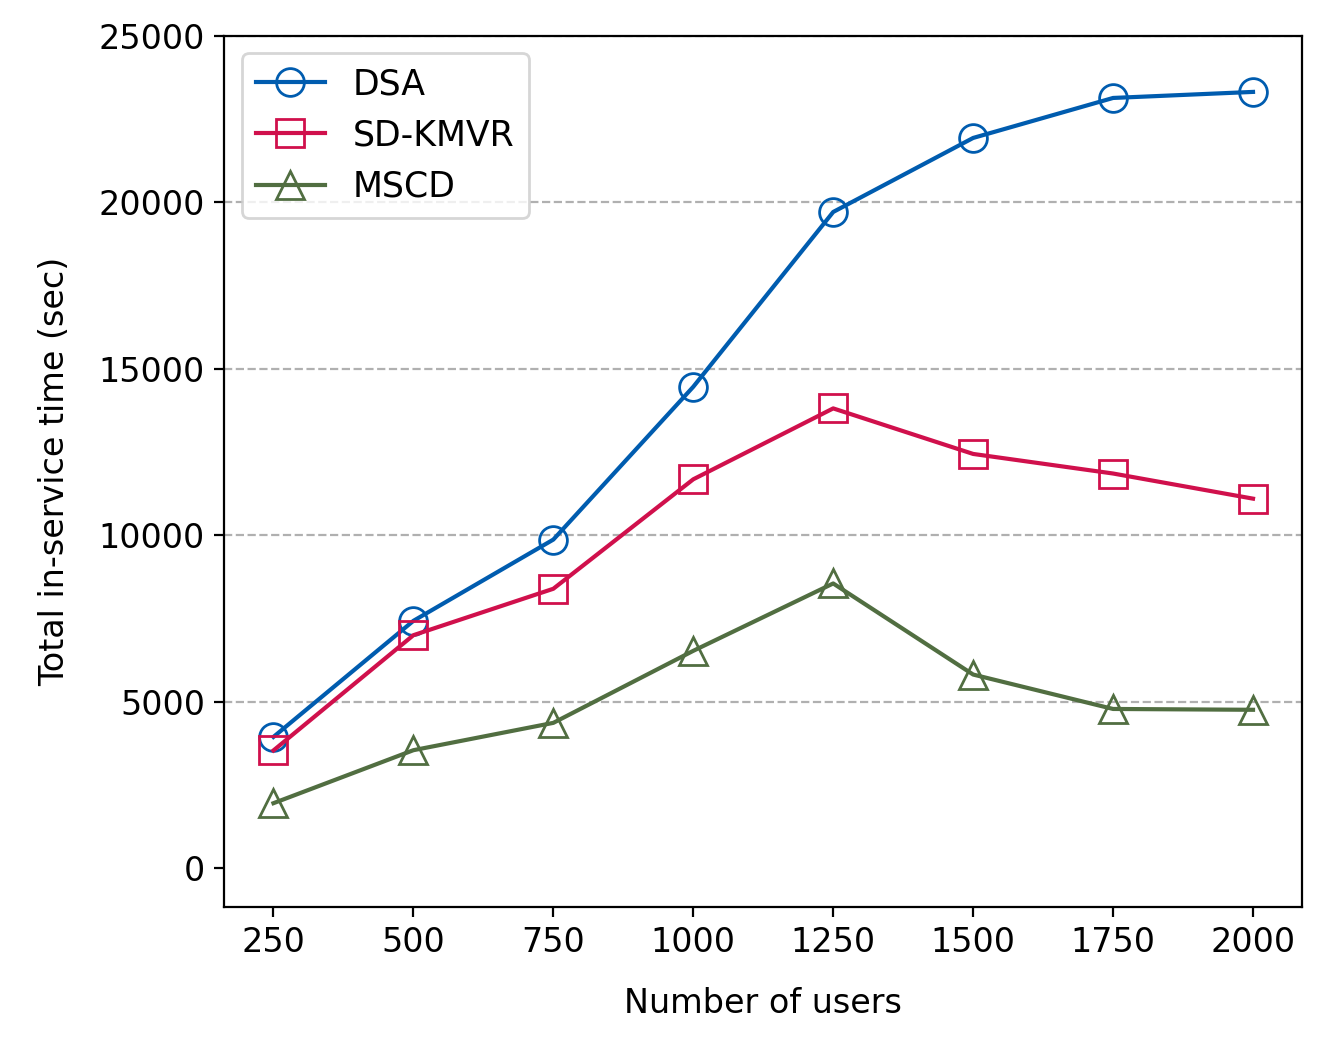
\includegraphics[width=0.7\textwidth]{Figure 5.png}
    \caption{Impact of the total in-service time under different numbers of users (with 8 service areas and 3 UAVs).}
    \label{fig:Impact on Total In-service Time}
\end{figure}
\begin{figure} [h!]
    \centering
    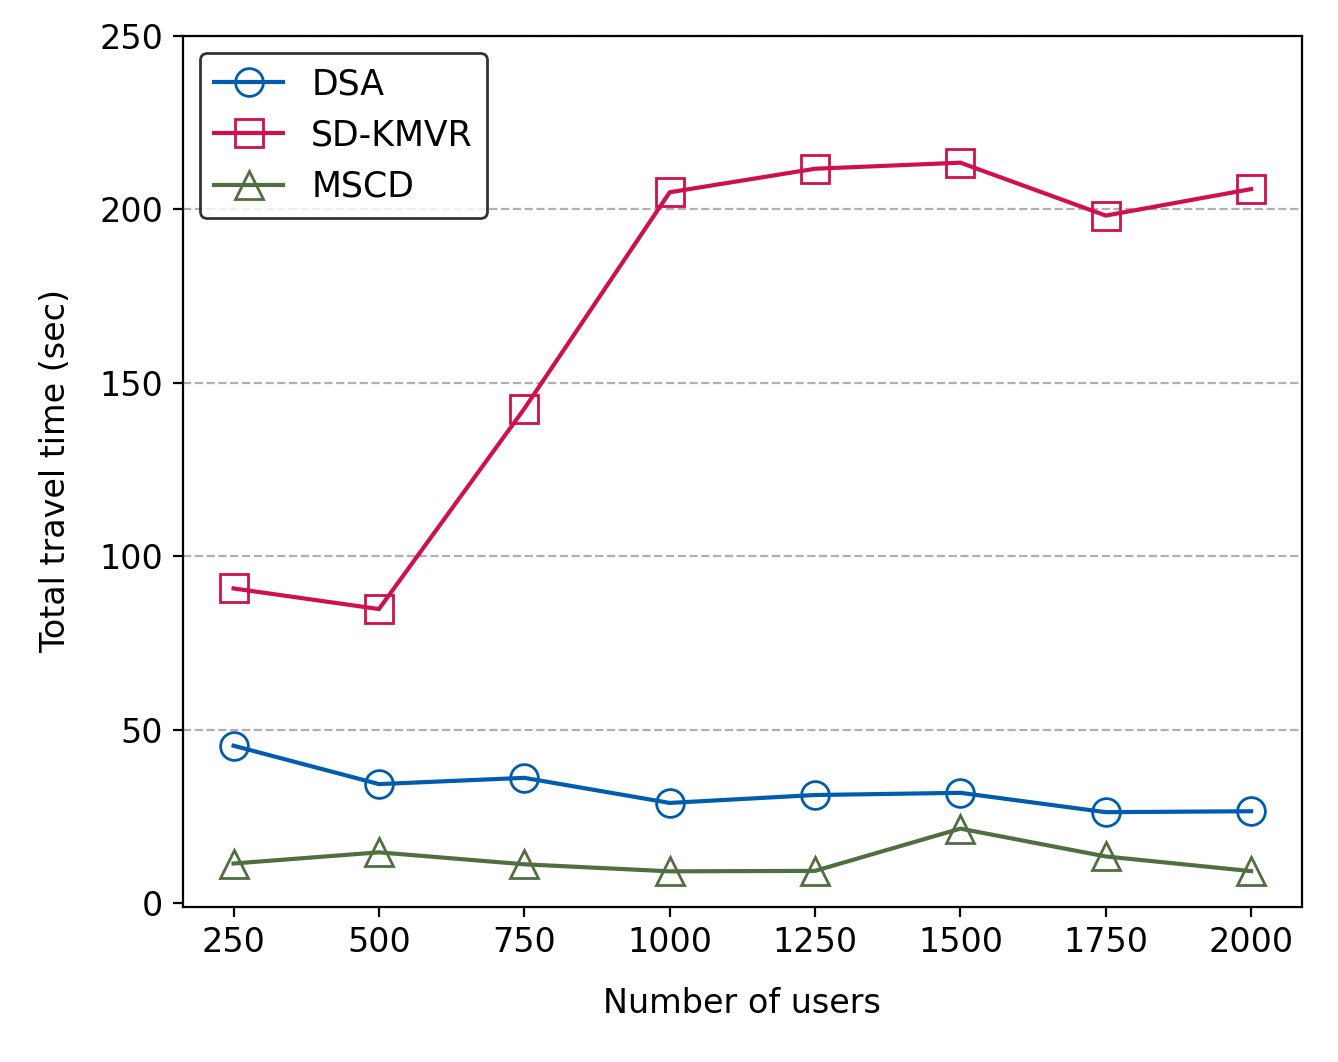
\includegraphics[width=0.7\textwidth]{Figure 6.png}
    \caption{Impacts of the total travel time under different numbers of users (with 8 service areas and 3 UAVs).}
    \label{fig:Impact on total travel time}
\end{figure}

\paragraph{}
Figure~\ref{fig:Impact on total travel time} depicts the total travel time by UAVs under different numbers of users. SD-KMVR has a longer total travel time than DSA and MSCD since it deploys UAVs based on the number of users served, which causes SD-KMVR to travel more frequently as the user's distribution changes over time. On the other hand, the overall travel time in DSA and MSCD is lower as they deploy UAVs by the in-service time that accounts for both the user's travel time and UAV's travel time, which can avoid unnecessary traveling by UAVs. Because MSCD uses non-moving predefined locations, MSCD has the lowest total UAV traveling time.

\begin{figure} [h!]
    \centering
    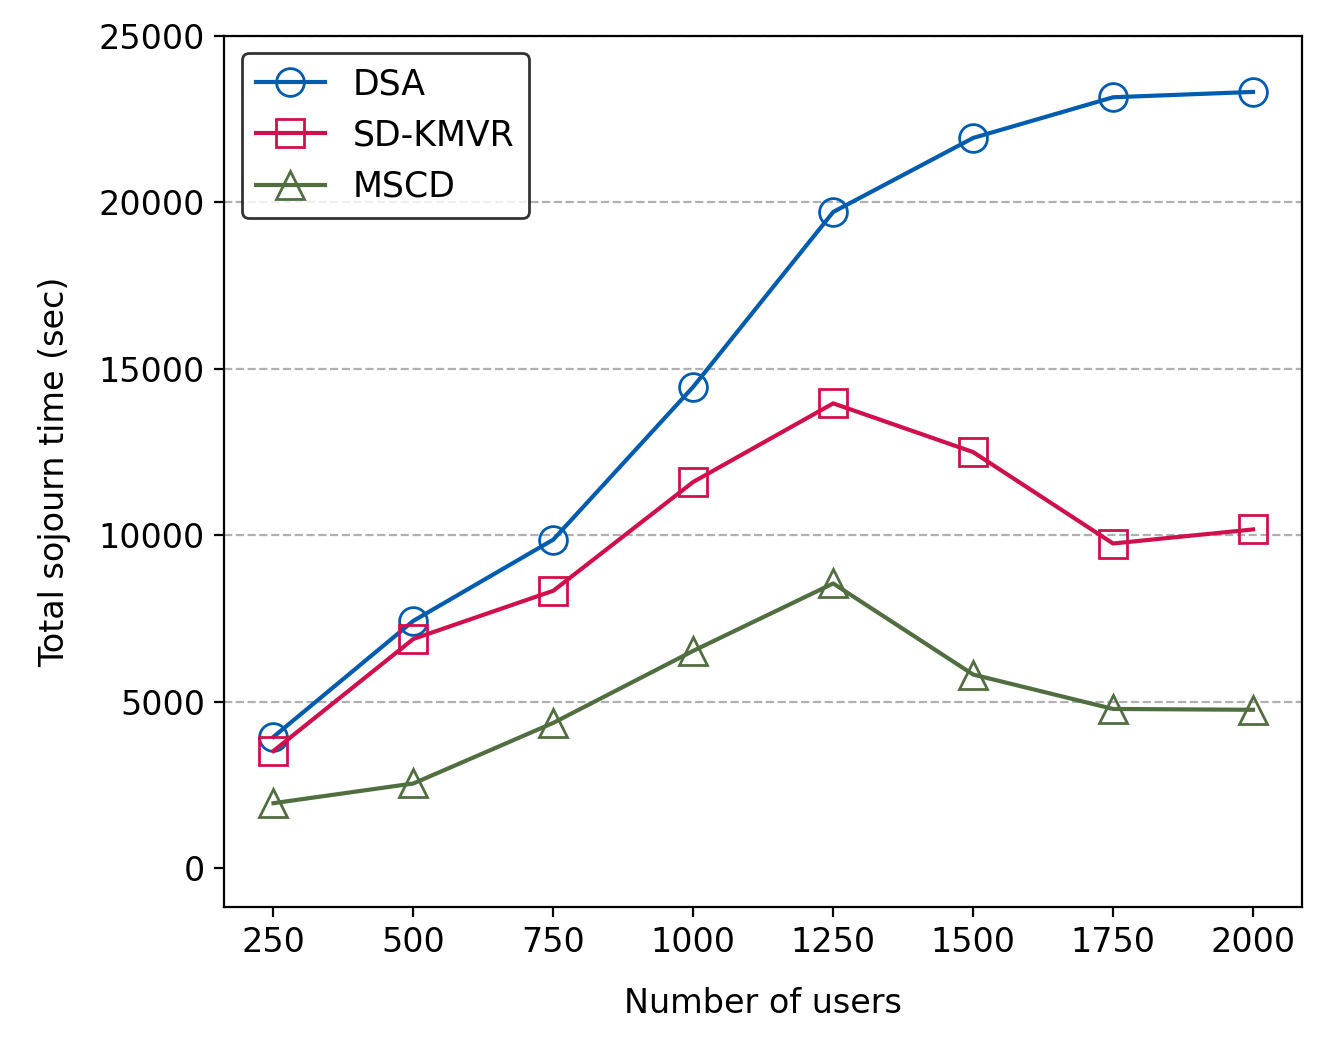
\includegraphics[width=0.7\textwidth]{Figure 7.png}
    \caption{Impacts of the total sojourn time under different numbers of users (with 8 service areas and 3 UAVs).}
    \label{fig:Impact on total sojourn time}
\end{figure}
\paragraph{}
Figure~\ref{fig:Impact on total sojourn time} investigates the total sojourn time served by UAVs under different numbers of users. In line with the result from Figure~\ref{fig:Impact on Total In-service Time}, DSA provides a higher total sojourn time across all given numbers of users. The total sojourn time of SD-KMVR and MSCD will not always increase because optimal service areas cannot always be chosen when the number of users increases. Despite SD-KMVR having a higher total sojourn time than MSCD, its total in-service time from Figure~\ref{fig:Impact on Total In-service Time} is close to MSCD. This is due to SD-KMVR's longer travel times, which reduces in-service time. As a result, we can observe the importance of considering travel time when deploying UAVs.

\begin{figure} [h!]
    \centering
    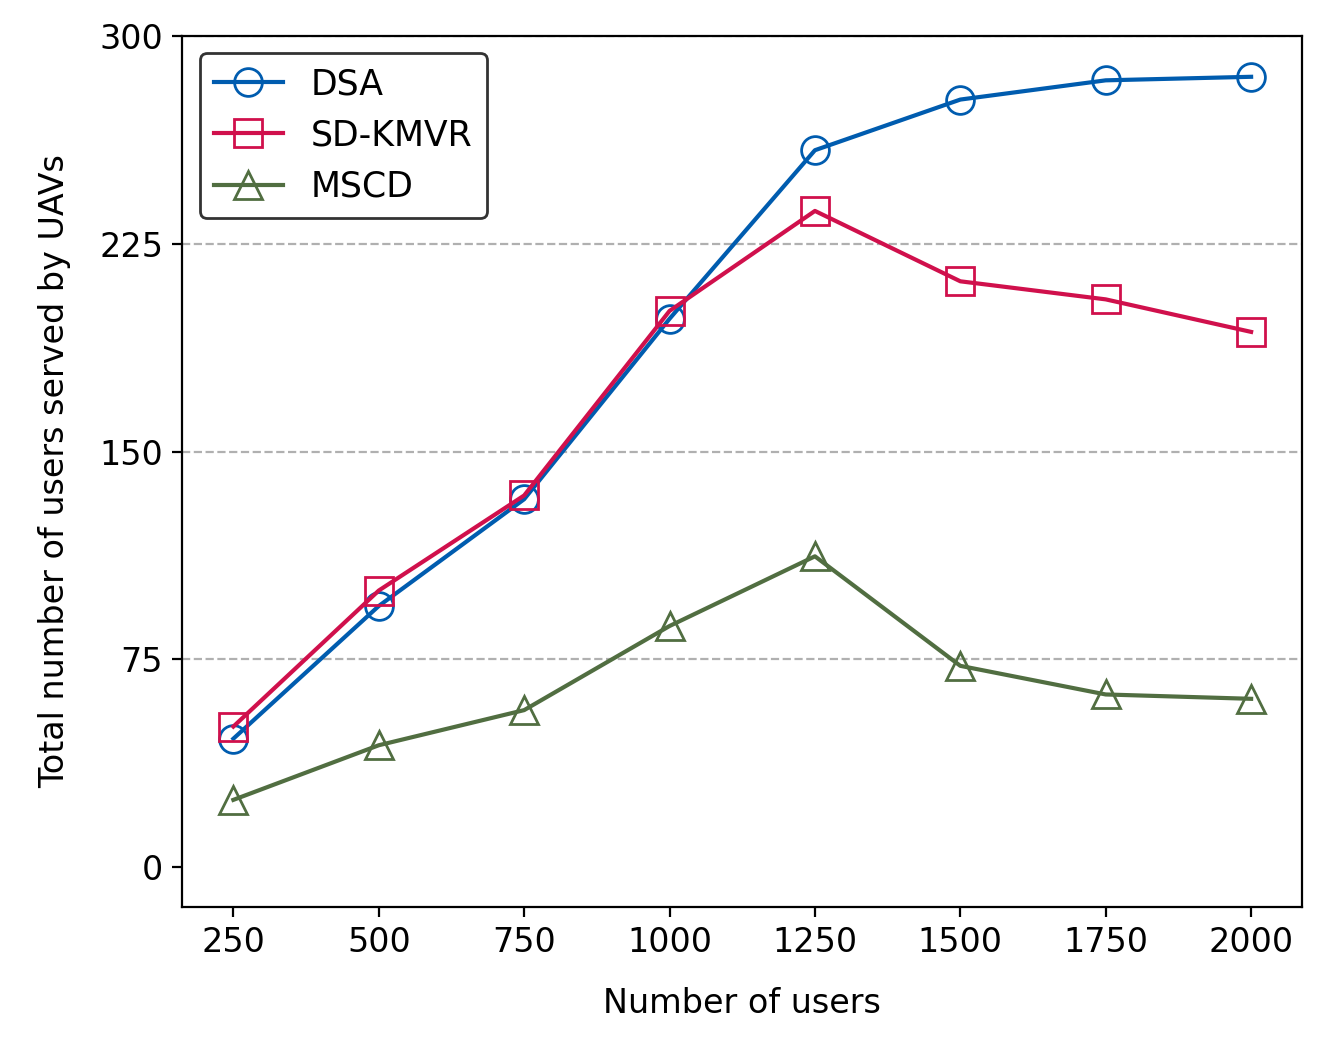
\includegraphics[width=0.7\textwidth]{Figure 8.png}
    \caption{Impact of the number of users served by UAVs under different numbers of users (with 8 service areas and 3 UAVs).}
    \label{fig:Impact on Number of Users Served by UAV}
\end{figure}
\paragraph{}
Figure~\ref{fig:Impact on Number of Users Served by UAV} shows the total number of users served by UAVs under different numbers of users. With DSA, when the number of users in the network rises, the number of users served by UAVs will also increase. By combining this result with Figure~\ref{fig:Impact on total sojourn time}, we can observe an interesting phenomenon that SD-KMVR and DSA are serving similar numbers of users before 1250 users, yet DSA can provide a higher total sojourn time. This result suggests that serving more users does not always lead to a higher total sojourn time. Some users served by SD-KMVR are likely to be traveling, thus contributing less to sojourn time.
\paragraph{}
Figure~\ref{fig:Impact on average radius} explores the average radius of all service areas under different numbers of users generated by three algorithms. DSA's radius won't increase as the number of users rises, since it will prevent serving too many users to meet their QoS requirements. SD-KMVR, however, aims to serve as many users as possible, which causes its radius to increase continuously. MSCD's average radius will always remain the same, due to having predefined locations with a constant radius. Combining the result from this Figure with Figure~\ref{fig:Impact on Total In-service Time}, we can observe that having a larger radius will not always lead to higher total in-service time. Moreover, DSA can provide higher total in-service time with a smaller radius, which can help it meet QoS requirements for users.
\begin{figure} [h!]
    \centering
    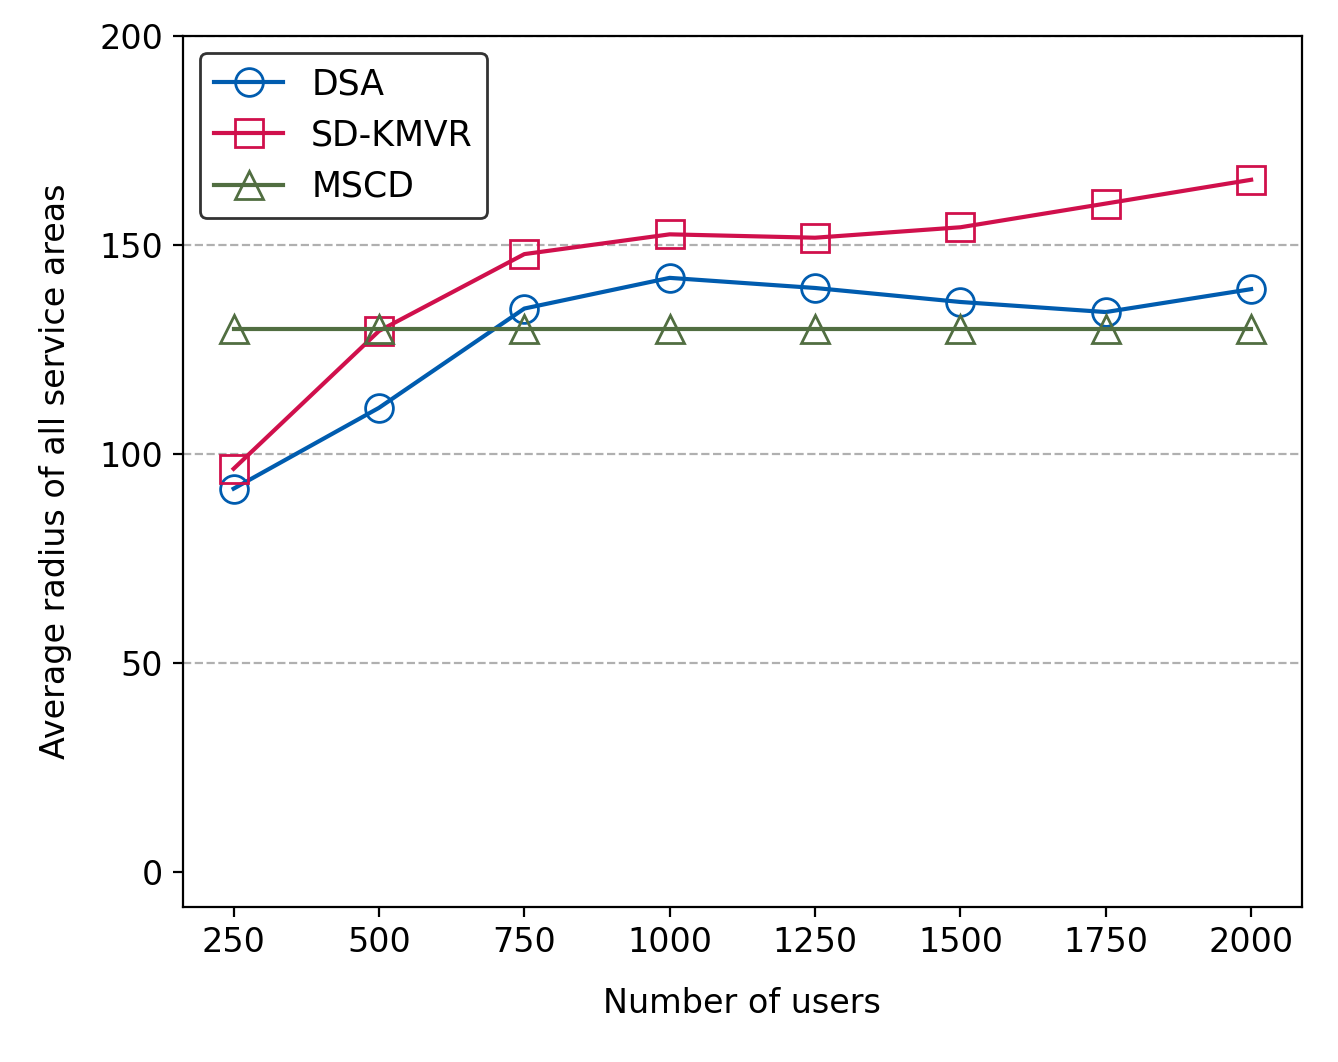
\includegraphics[width=0.7\textwidth]{Figure 9.png}
    \caption{Impacts of the average radius of all service areas under different numbers of users (with 8 service areas and 3 UAVs).}
    \label{fig:Impact on average radius}
\end{figure}

\paragraph{}
Figure~\ref{fig:Impact on total in-service time with different numbers of SA} illustrates the total in-service time provided by UAVs under the different number of service areas with 2000 users. DSA and SD-KMVR will have a lower impact on total in-service time as they will move to find the optimal placement of service areas in each region. However, MSCD's total in-service time increases with the increase in service areas since it utilizes predefined locations that are static. With the expansion in service areas in MSCD, UAVs can have more choices and provide higher total in-service time. This result shows the importance of generating service areas by moving within each region, which can help to ensure the most optimal placement of service areas.
\begin{figure} [h!]
    \centering
    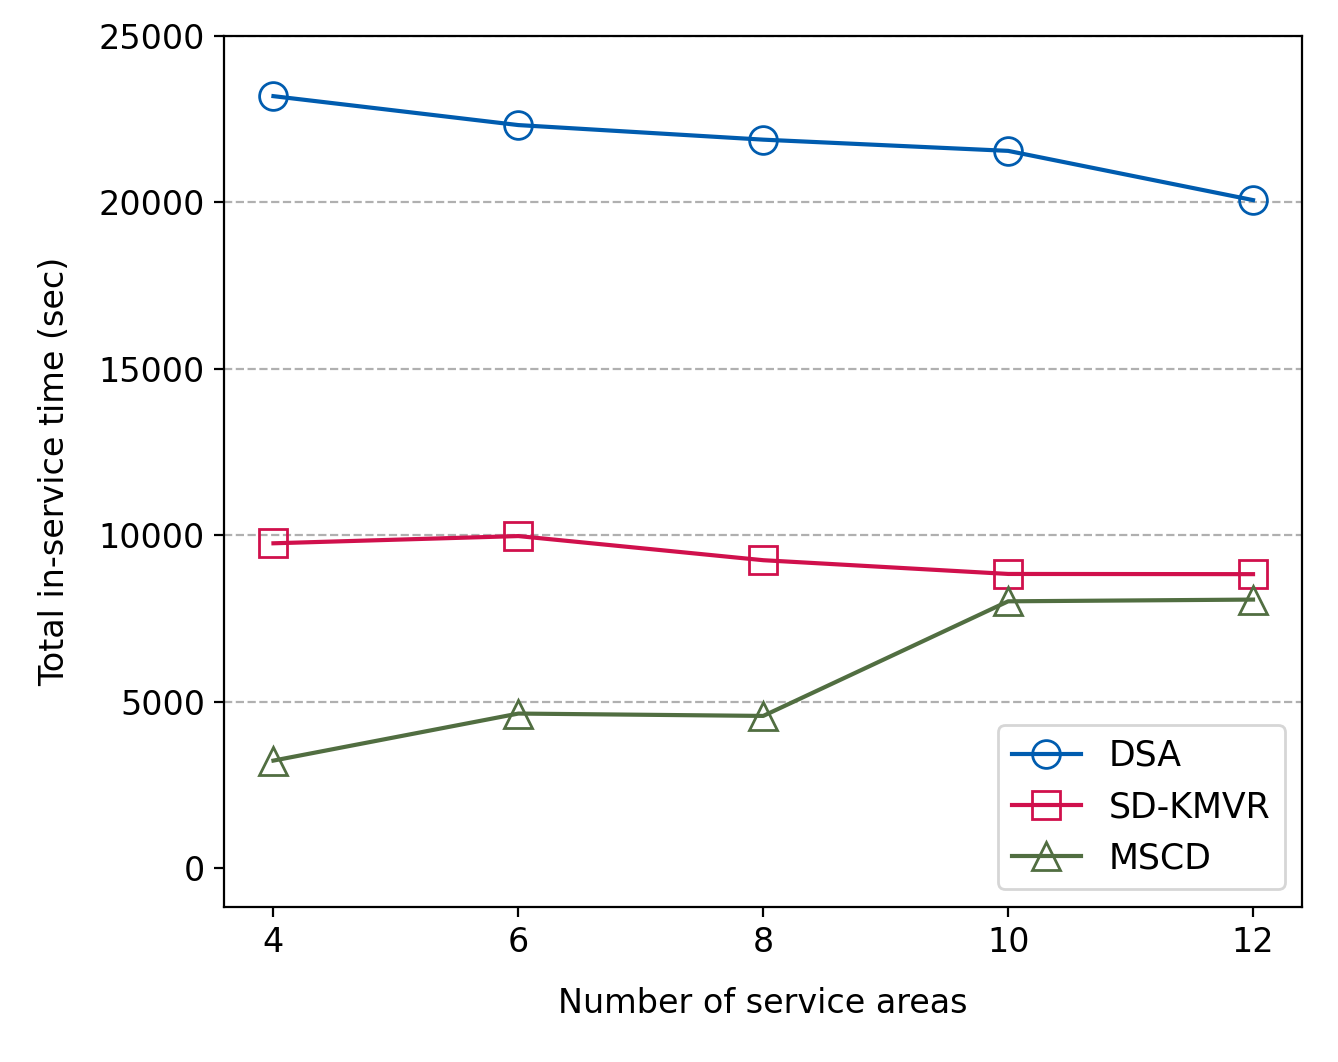
\includegraphics[width=0.7\textwidth]{Figure 10.png}
    \caption{Impact on total in-service time under different numbers of service areas (with 2000 users and 3 UAVs).}
    \label{fig:Impact on total in-service time with different numbers of SA}
\end{figure}

\paragraph{}
\begin{figure} [h!]
    \centering
    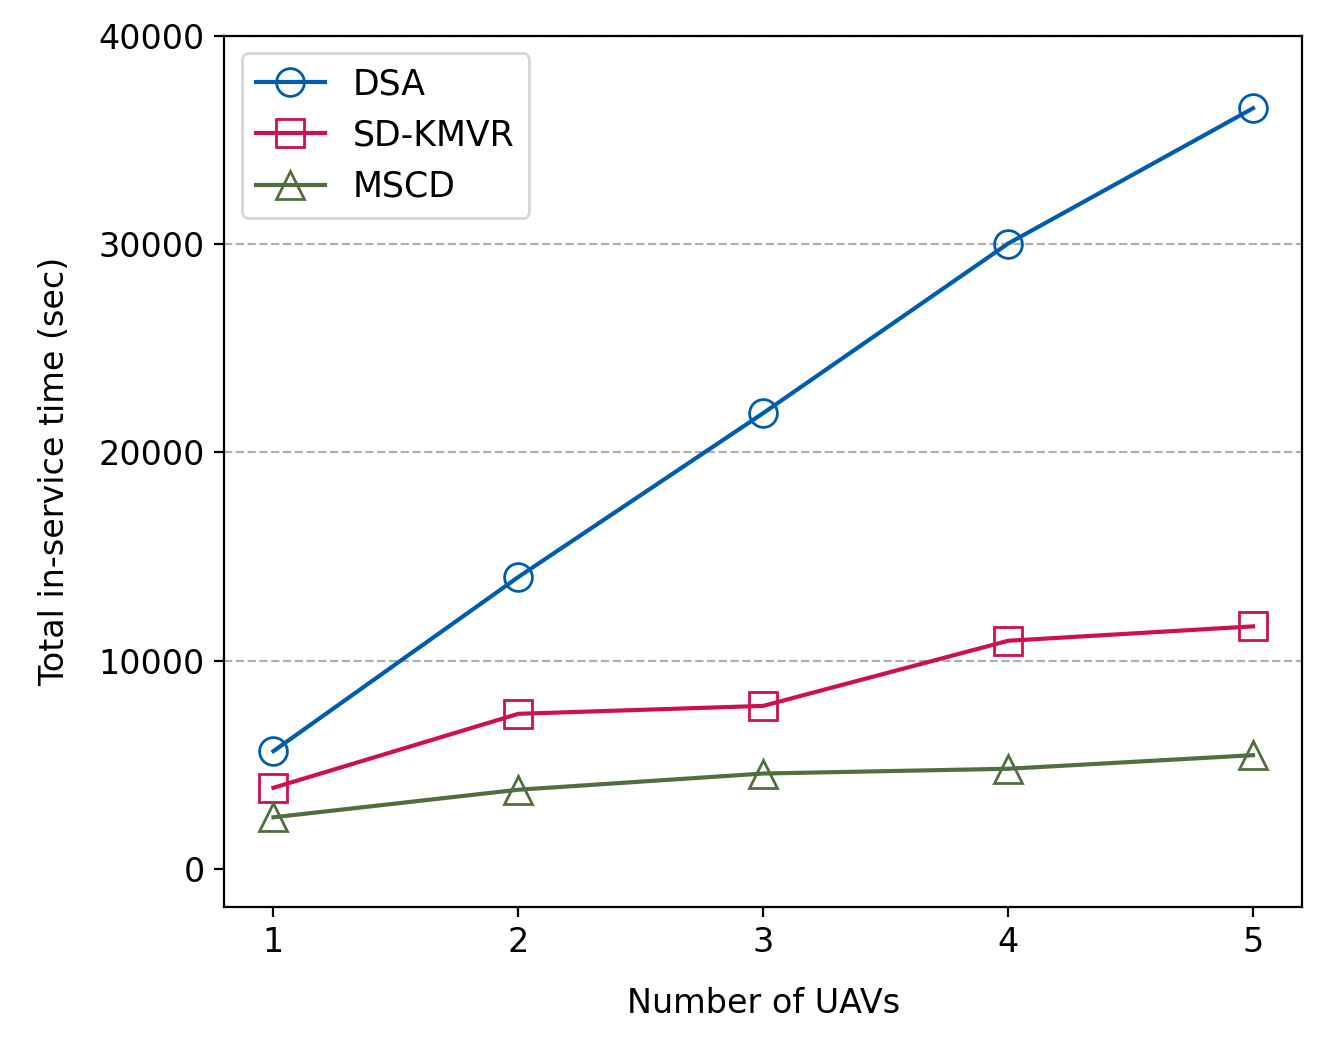
\includegraphics[width=0.7\textwidth]{Figure 11.png}
    \caption{Impact on total in-service time under different numbers of UAVs (with 2000 users and 8 service areas).}
    \label{fig:Impact on total in-service time with different numbers of UAVs}
\end{figure}
Figure~\ref{fig:Impact on total in-service time with different numbers of UAVs} shows the impact on total in-service time with different numbers of UAVs with 2000 users. As the number of UAVs increases, DSA will increase as more UAVs are available to provide services to users. SD-KMVR and MSCD do not produce significant increases in in-service time compared to DSA due to their inability to meet all users' requirements in some generated service areas. Due to this, the total in-service time isn't increased in spite of the increase in the number of UAVs available. This result also illustrates the necessity of considering all serving users' QoS needs when generating service areas.

\begin{figure} [h!]
    \centering
    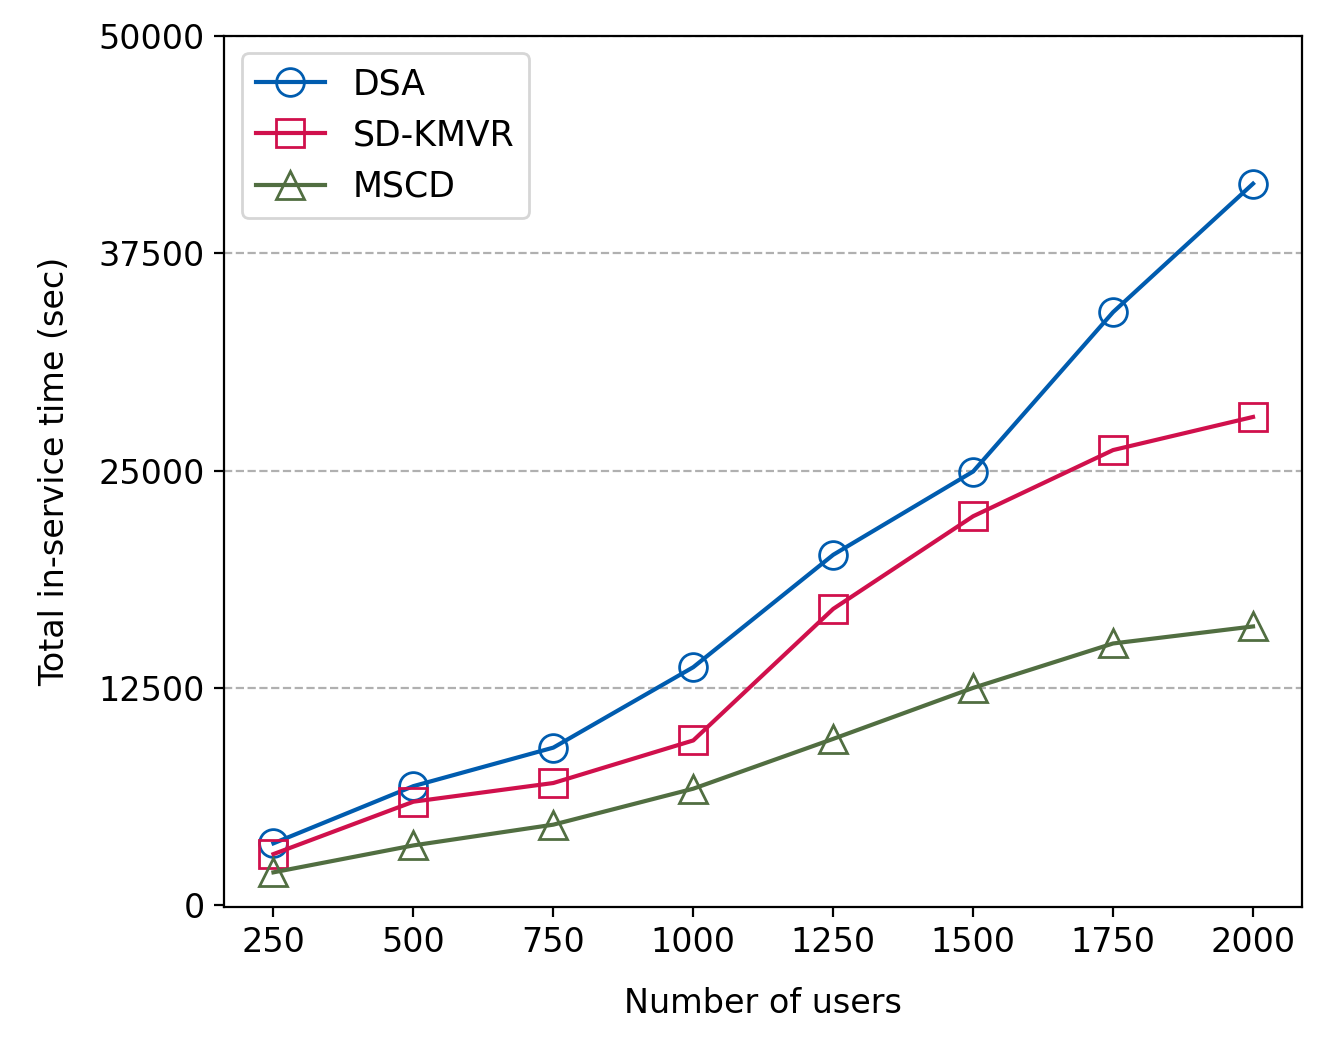
\includegraphics[width=0.7\textwidth]{Figure 12.png}
    \caption{Impact on total in-service time under different numbers of users with 1 Mbps QoS requirement (with 8 service areas and 3 UAVs).}
    \label{fig:Impact on total in-service time under different numbers of users with 1 Mbps QoS requirement}
\end{figure}
\paragraph{}
Figure~\ref{fig:Impact on total in-service time under different numbers of users with 1 Mbps QoS requirement} present the impact on total in-service time under different numbers of users. In this simulation, the in-service result is also tested with a different number of users, however, the difference from Figure~\ref{fig:Impact on Total In-service Time} is that all users only require web browsing for their QoS needs, which is 1 Mbps. Similar to Figure~\ref{fig:Impact on Total In-service Time}, DSA performs the best among the three algorithms in terms of in-service time. The main difference from Fig.5 is that all three algorithms will increase as the number of users increases, and SD-KMVR and MSCD will not decrease after 1250 users. The reduced QoS requirement allows SD-KMVR and MSCD to meet the QoS requirements for more users when users increase. Combining the result with Figure~\ref{fig:Impact on Total In-service Time} we can observe the impact on the user's QoS requirement in in-service time.

\chapter{Conclusion}
\paragraph{}
This paper studies the 3D deployment of UAVs to provide communication services for users in disaster areas. We propose the DSA algorithm to solve the deployment problem effectively. In our proposed scheme, users' service time and QoS are taken into account jointly. Moreover, we generate service areas by moving and increasing the radius in Voronoi regions to adapt to the changing user distribution. Each service area's height is also dynamically selected by the distance between users and the UAV to ensure the optimal connection between the UAV and users.
\paragraph{}
The simulation results show that our proposed scheme can successfully find the trade-off between in-service time and satisfying users' QoS requirements. We also observe the importance of considering UAV's travel time and users' sojourn time while deploying UAVs. Additionally, we have also discovered that serving more users and having a larger radius does not always result in higher in-service time.

\newpage
\addcontentsline{toc}{chapter}{Bibliography}
\bibliographystyle{IEEEtran}
\bibliography{references}

\end{document}
